\section{Modelo de información del sistema}
En la Figura \ref{fig:Base_ServidorEmbebido} se observa un diagrama del modelo de información correspondiente al repositorio de datos almacenado en el servidor embebido, se puede observar que las tablas no se encuentran relacionadas porque no existe relación alguna entre los datos, cada tabla representa un archivo JSON, cada nodo sensor tiene este conjunto de archivos en una carpeta contenedora, esto ayuda a identificar entre los 4 diferentes direcciones de sensores posibles, donde el sensor es identificado por su número de esclavo (0 al 3), los microcontroladores se identifican por su número de serie, contienen a los sensores esclavos pertenecientes al microcontrolador y este a su vez está contenido por una carpeta que indica a que IP pertenece el microcontrolador, por dar un ejemplo, 192.168.0.3/AA/0 indicaría que el servidor con IP 192.168.0.3 contiene al microcontrolador con número de serie AA y tiene un sensor con número de esclavo 0. 
\paragraph{}
Cada archivo JSON representa un arreglo de objetos con los atributos como se especifican en la figura \ref{fig:Base_ServidorEmbebido}\\
En el archivo de tiempo real se guarda el valor de los parámetros obtenidos cada segundo, sobrescribiéndolo en ese mismo tiempo.
\\
En las muestras del día, se almacenarán un total de 1440 objetos con los atributos especificados, es decir se almacenará una muestra por minuto para poder generar la gráfica de producción del día.
\\
Al finalizar el día, también se guarda una copia de estas muestras como muestras de ayer, con el propósito de poder graficar el comportamiento de la producción un día anterior si el usuario lo desea.
\\
En las muestras del mes, se almacena la información de generación de energía de los 28, 29, 30 ó 31 días del mes.
\\
En las muestras del año, se almacenan los 12 valores de generación de energía de cada mes del año.
\\
Por último, se  almacenan los valores de generación de cada mes, de cada año, por diez años.

\begin{figure}[H]
	\centering
	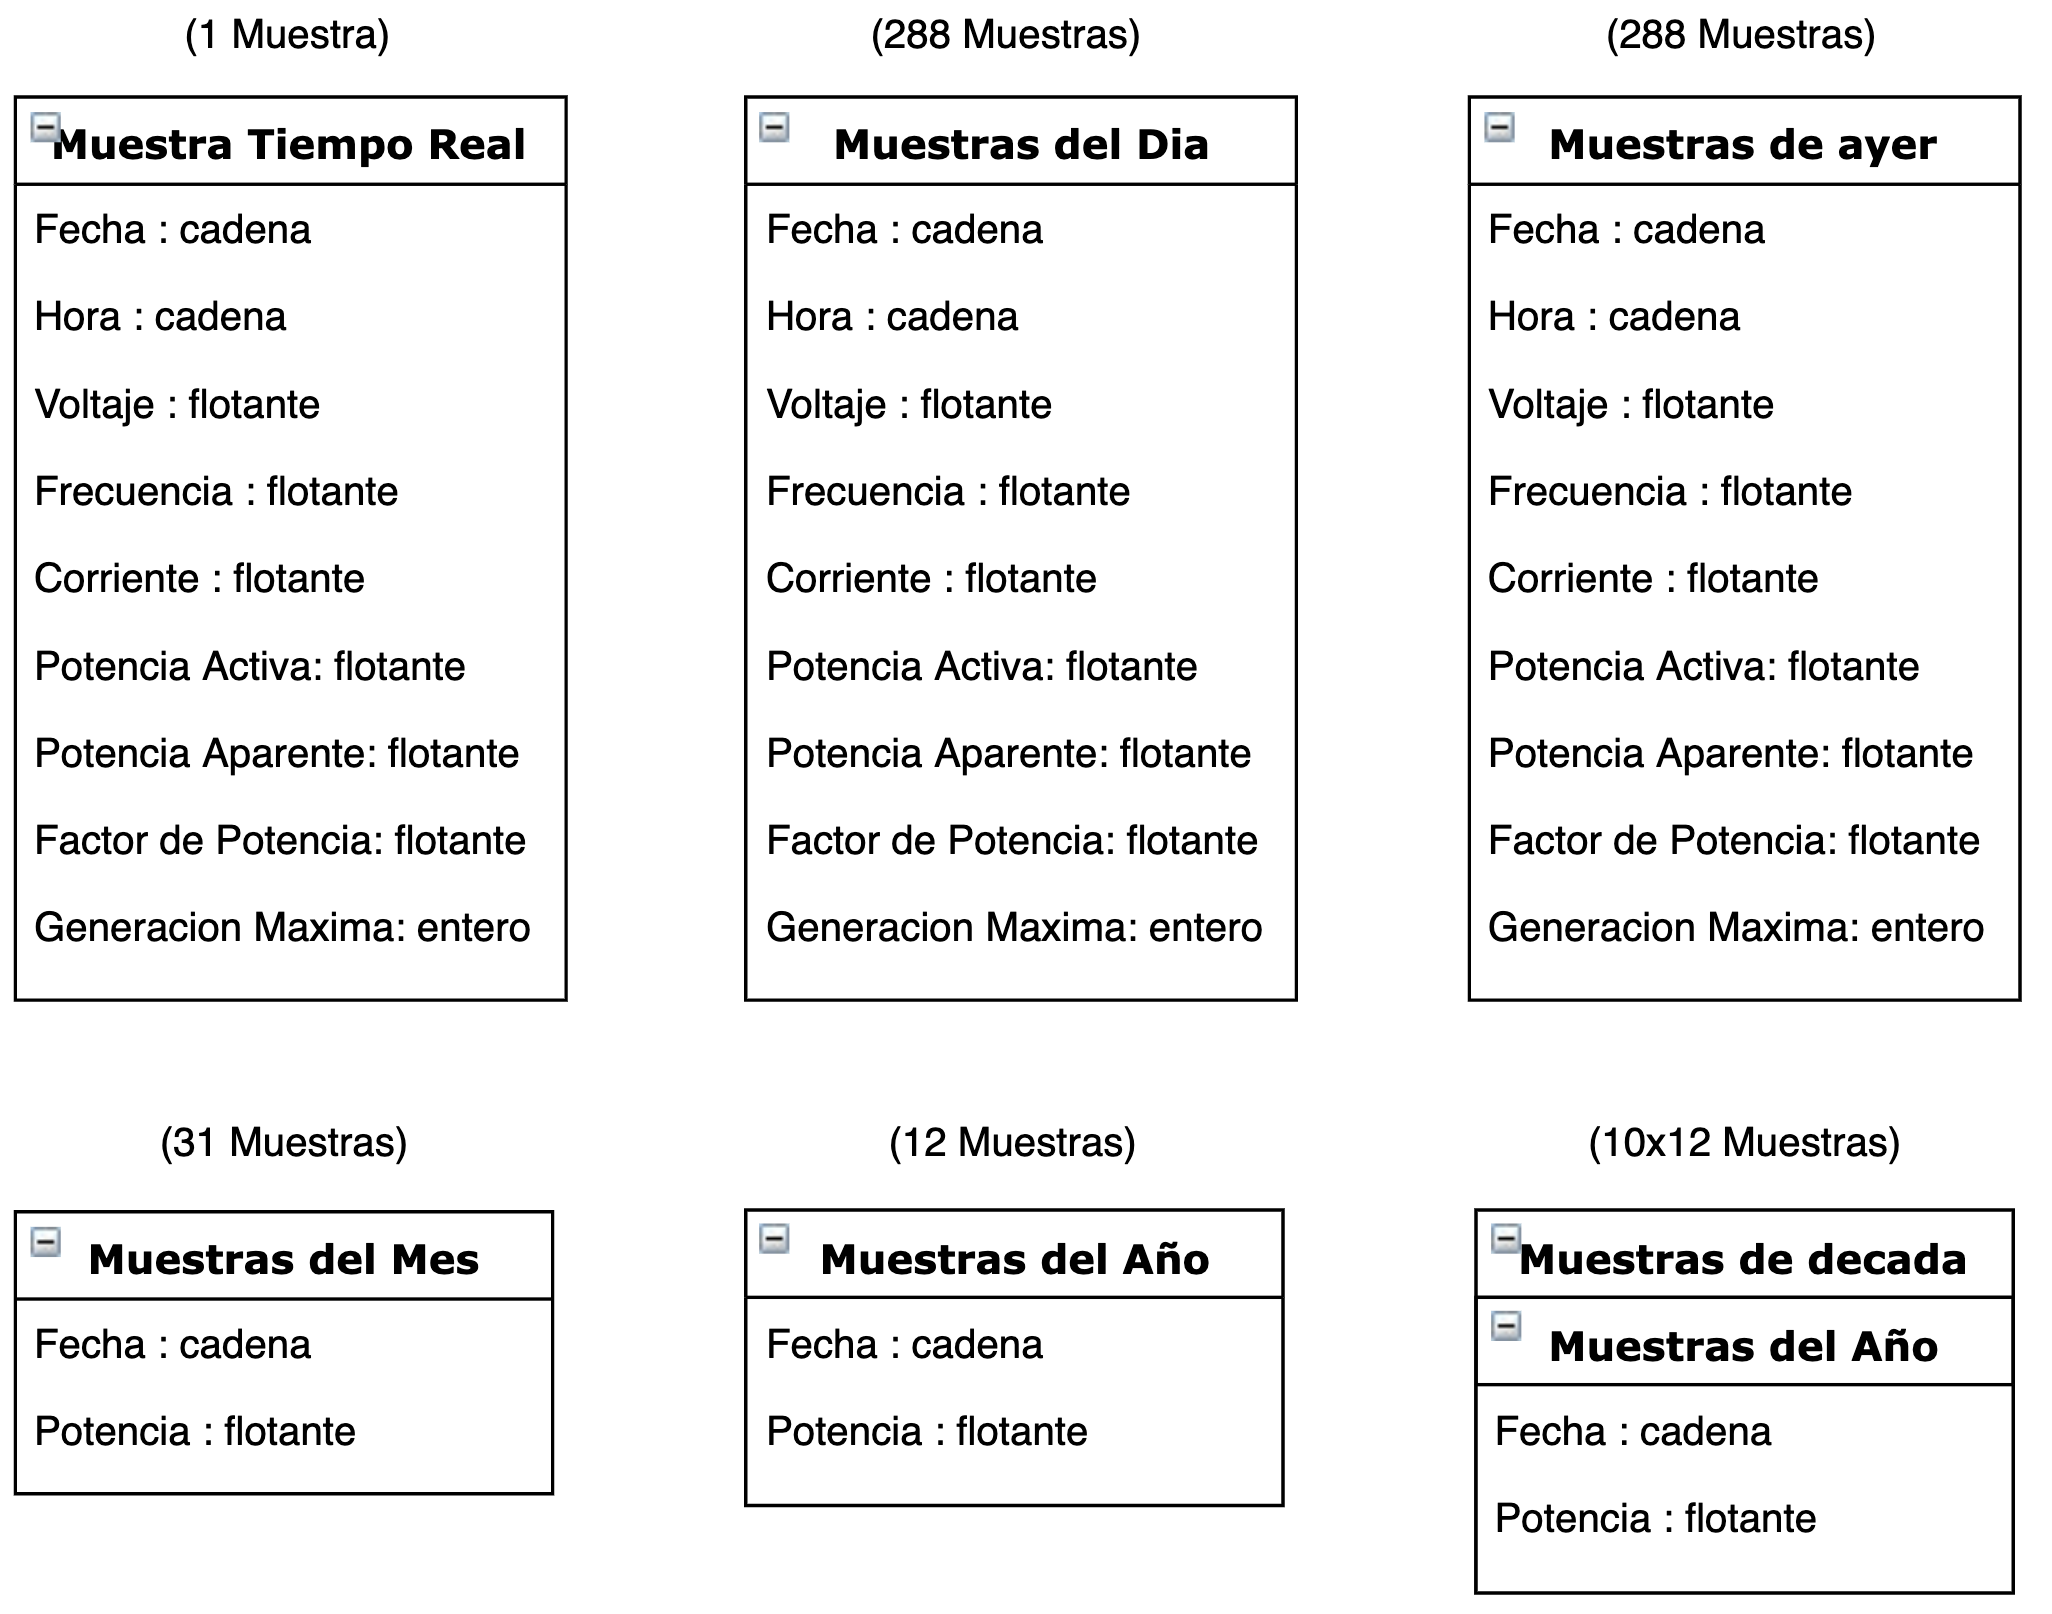
\includegraphics[scale=.30]{Capitulo4/images/Base_ServidorEmbebido.png}
	\caption{Modelo de información del Servidor Embebido}
	\label{fig:Base_ServidorEmbebido}
\end{figure}

A continuación en la Figura \ref{fig:Base_AplicacionUsuario} se muestra el diagrama del modelo de información correspondiente a la aplicación de usuario, en donde se puede observar que se almacenarán las notificaciones y los servidores que den respuesta a las peticiones de la aplicación de usuario. La relación entre tablas nos indica que muchas notificaciones pueden pertenecer a un mismo servidor.
\\
El archivo en el que se almacenarán las notificaciones recibidas durante el proceso de monitoreo de los nodos conectados al servidor, será un archivo JSON; este archivo a lo más contendrá las últimas 100 notificaciones recibidas, es decir, cuando se tengan 100 notificaciones y se cree una nueva notificación, se reemplazará la notificación más antigua para almacenar la nueva notificación. 

\begin{figure}[H]
	\centering
	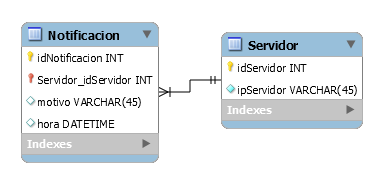
\includegraphics[scale=0.8]{Capitulo4/images/Base_AplicacionUsuario.PNG}
	\caption{Modelo de información de la aplicación de usuario}
	\label{fig:Base_AplicacionUsuario}
\end{figure}